\setcounter{secnumdepth}{1}

\chapter{Lab 1}

\section{DFT}

\begin{Task}{Task 1.1.1.}
    Prove that
    \begin{equation*}
        \omega_k = \frac{2\pi}{T} k
    \end{equation*}
    where $T = nT_s$ is the window length.
\end{Task}

Starting from the general definition of the iDFT and the one in case of a discrete signal:

\begin{align*}
    x(n) = \frac{1}{N} \sum_{k=0}^{N-1} X(k) e^{\frac{j 2 \pi k n}{N}}\\
    x(n) = \frac{1}{N} \sum_{k=0}^{N-1} X(k) e^{j \omega_k n T_s}
\end{align*}

By simply comparing both equations, $\omega_k = \frac{2\pi}{n T_s} k$. Replacing the sampling period $T_s$ multiplied with the number of samples $n$ by the total sampling time, the result is obtained.

\begin{equation*}
    \omega_k = \frac{2\pi}{T} k
\end{equation*}

\begin{Task}{Task 1.1.2.}
    Prove that
    \begin{equation*}
        \omega_1 = \frac{2\pi}{T} = 2\pi \frac{f_s}{N}
    \end{equation*}
\end{Task}

The first equality is proven using the result of the previous task. By replacing $T$ the window length by $nT_s$ and then defining the sampling frequency $f_s = \frac{1}{T_s}$, the result is obtained.

\begin{Task}{Task 1.1.3.}
    Prove that
    \begin{equation*}
        X(N-k) = X(-k) = X^*(k)
    \end{equation*}
    \textit{Hint: Use $e^{j2\pi n} = 1$ for n $\in \mathbb{N}$ and $x(n) \in \mathbb{R}$.}
\end{Task}

By using the definition of the DFT, the following equation is obtained:

\begin{align*}
    X(k) = \sum_{n=0}^{N-1} x(n) e^{\frac{-j2\pi kn}{N}}\\
    X(N-k) = \sum_{n=0}^{N-1} x(n) e^{\frac{-j2\pi Nn}{N}-\frac{-j2\pi kn}{N}}\\
    X(N-k) = \sum_{n=0}^{N-1} x(n) e^{\frac{j2\pi kn}{N}}\\
\end{align*}

Where the last equality is obtained by removing the term $e^{-j2\pi n}$ which is equal to 1. By finally comparing the first and the third equation, one can see that only a minus sign is missing. Either $k$ is replaced by $-k$ giving:

\begin{equation*}
    X(N-k) = X(-k)
\end{equation*}

Either the conjugate of the whole equation is taken (needing the assumption that $x(n) \in \mathbb{R}$):

\begin{equation*}
    X(N-k) = X^*(k)
\end{equation*}

\section{DFT of a (co)sine}

\begin{Task}{Task 1.2.1. DFT of a 3 periods cosine}
    Generate a cosine sequence in Matlab with a randomly selected phase, and with a period that fits exactly 3 times in a data sequence of N = 1000 samples. Make a plot of the DFT of this sequence (amplitude and phase).
\end{Task}

\begin{figure}[H]
    \centering
    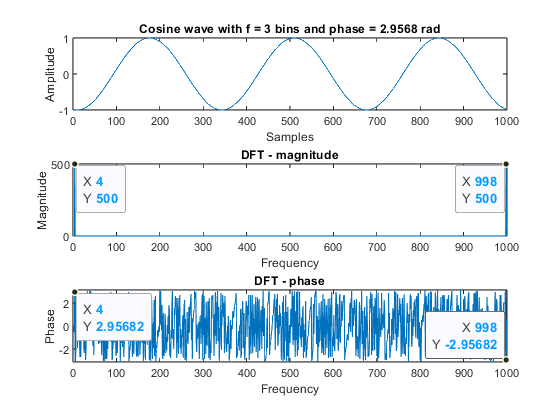
\includegraphics[width=1\textwidth]{part1/task1_2_1.png}
    \caption{DFT of a 3 periods cosine}
\end{figure}

Remarks: from the previous section, it is known that the DFT of a cosine at a frequency of 3 bins would create a peak at the third bin and one at the N - 3 bin as $X(N-k) = X^*(k)$. There is a shift of 1 bin as matlab indices starts at 1. concerning the phase plot, the phase at the third bin is indeed the one chosen randomly. The phases at the other bins are not relevant as the cosine is not present at these frequencies. The phase at the N - 3 bin is the opposite of the one at the third bin as $X(N-k) = X^*(k)$.

\begin{Task}{Task 1.2.2. Perfect reconstruction}
    From the DFT plot, check that the condition for perfect reconstruction is satisfied. Is there any leakage visible?\\
    \textit{Hint: use a logarithmic amplitude axis to distinguish small (but non-zero) values.}
\end{Task}

\begin{figure}[H]
    \centering
    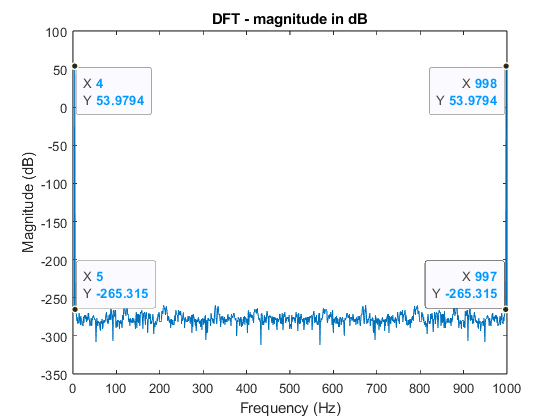
\includegraphics[width=1\textwidth]{part1/task1_2_2.png}
    \caption{Perfect reconstruction}
\end{figure}

There is a difference in amplitude of more than 300 dB between the excited bin and its neighbors. This shows that the condition for perfect reconstruction is satisfied.

\begin{Task}{Task 1.2.3. Intrpretation of the frequency axis}
    At which indices of the DFT do you obtain non-zero values? Explain. (Keep in mind that Matlab indices start at 1, not at 0.)
\end{Task}

As already discussed in task 1.2.1, the DFT of a cosine at a frequency of 3 bins would create a peak at the third bin and one at the N - 3 bin as $X(N-k) = X^*(k)$. There is a shift of 1 bin as matlab indices starts at 1. The other bins are (close to) zero as there is no excitations at these frequencies.

\begin{Task}{Task 1.2.4. Frequency axis in bins}
    Construct the frequency axis for the plots, expressed in bins.
\end{Task}

It is already done in the matlab script as the x-axis of the plots is expressed in "DFT samples number", which are in fact bins.

\begin{Task}{Task 1.2.5. Frequency axis in Hz}
    Consider that the sample frequency is fs = 100 Hz. Construct the frequency axis for the plots, expressed in Hz.\\
    \textit{(Hint: use the results from Task 1.1.1.)}
\end{Task}

\begin{figure}[H]
    \centering
    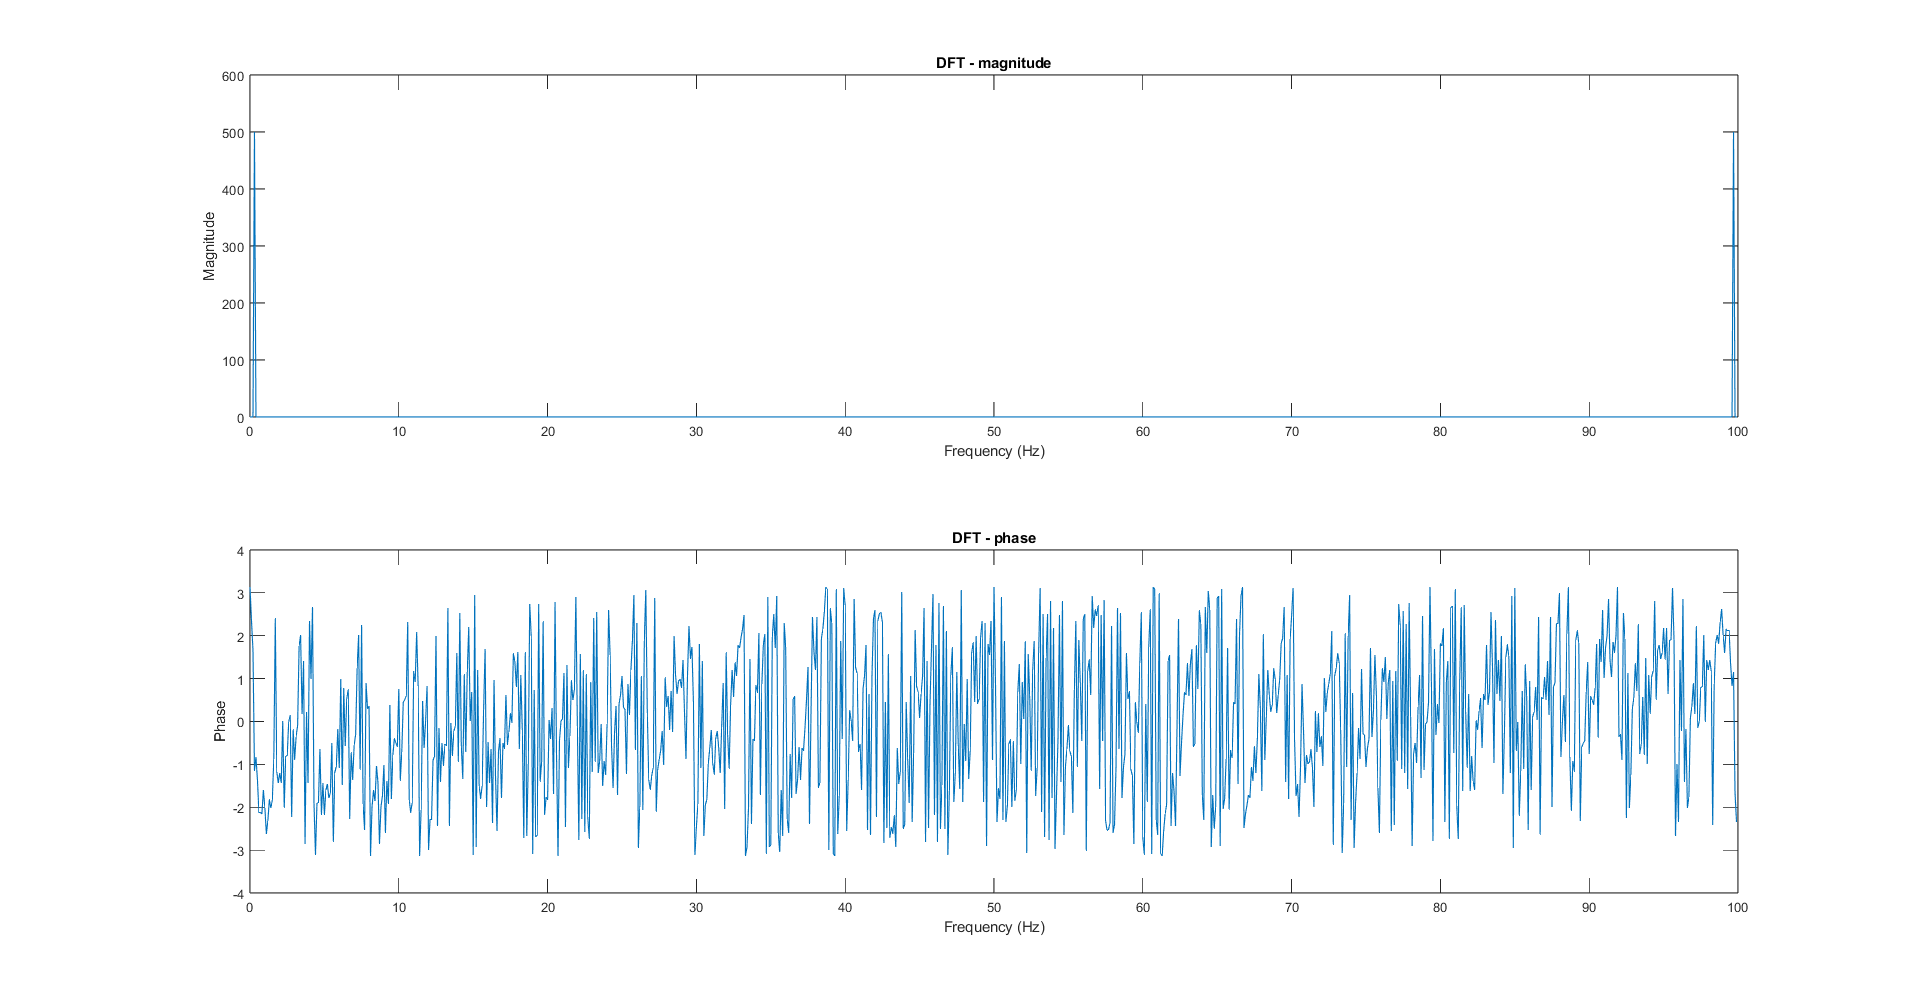
\includegraphics[width=1\textwidth]{part1/task1_2_5.png}
    \caption{Frequency axis in Hz}
\end{figure}

To change the frequency axis from bins to Hz, it was simply multiplied by $\omega_1 = \frac{f_s}{N}$.

\section{Time domain construction of a multisine}

\begin{Task}{Task 1.3.1. Time domain random phase multisine}
    Generate a multisine in the time domain, by implementing (1.6), with $N = 1000$ samples and $K = 10$ excited frequencies. Set the amplitudes $A_m = 1$, and choose the phases $\varphi_m$ randomly between $0$ and $2\pi$ (i.e. a random phase multisine). Check that this multisine satisfies the condition for perfect reconstruction by plotting its DFT. (Use a logarithmic amplitude axis). Include the frequency axis, expressed in bin.
\end{Task}

\begin{figure}[H]
    \centering
    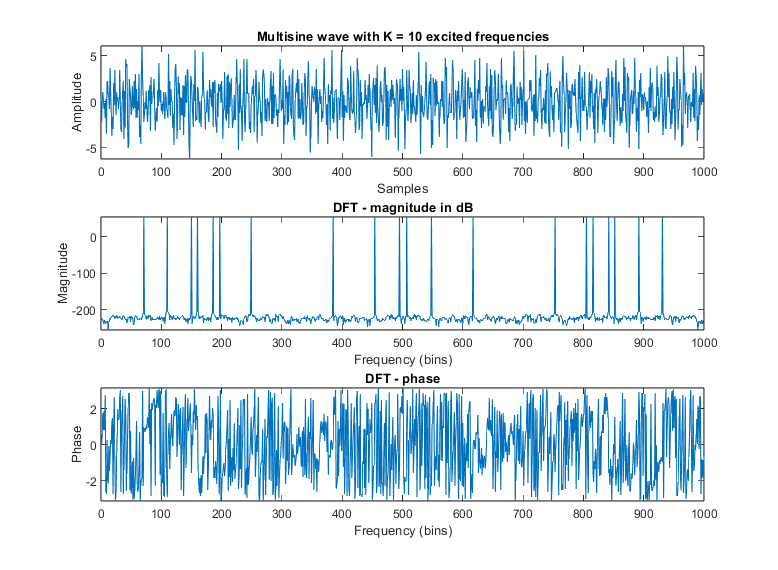
\includegraphics[width=1\textwidth]{part1/task1_3_1.png}
    \caption{Time domain random phase multisine}
\end{figure}

The condition for perfect reconstruction is satisfied as the difference in amplitude between the excited bins and their neighbors is more than 250 dB.

\begin{Task}{Task 1.3.2. Frequency axis in Hz}
    For the multisine generated in Task 1.3.1, consider that the sampling frequency is $f_s = 100 Hz$. Include the frequency axis expressed in Hz in the DFT plot, and the time axis expressed in seconds for the time domain plot.
\end{Task}

\begin{figure}[H]
    \centering
    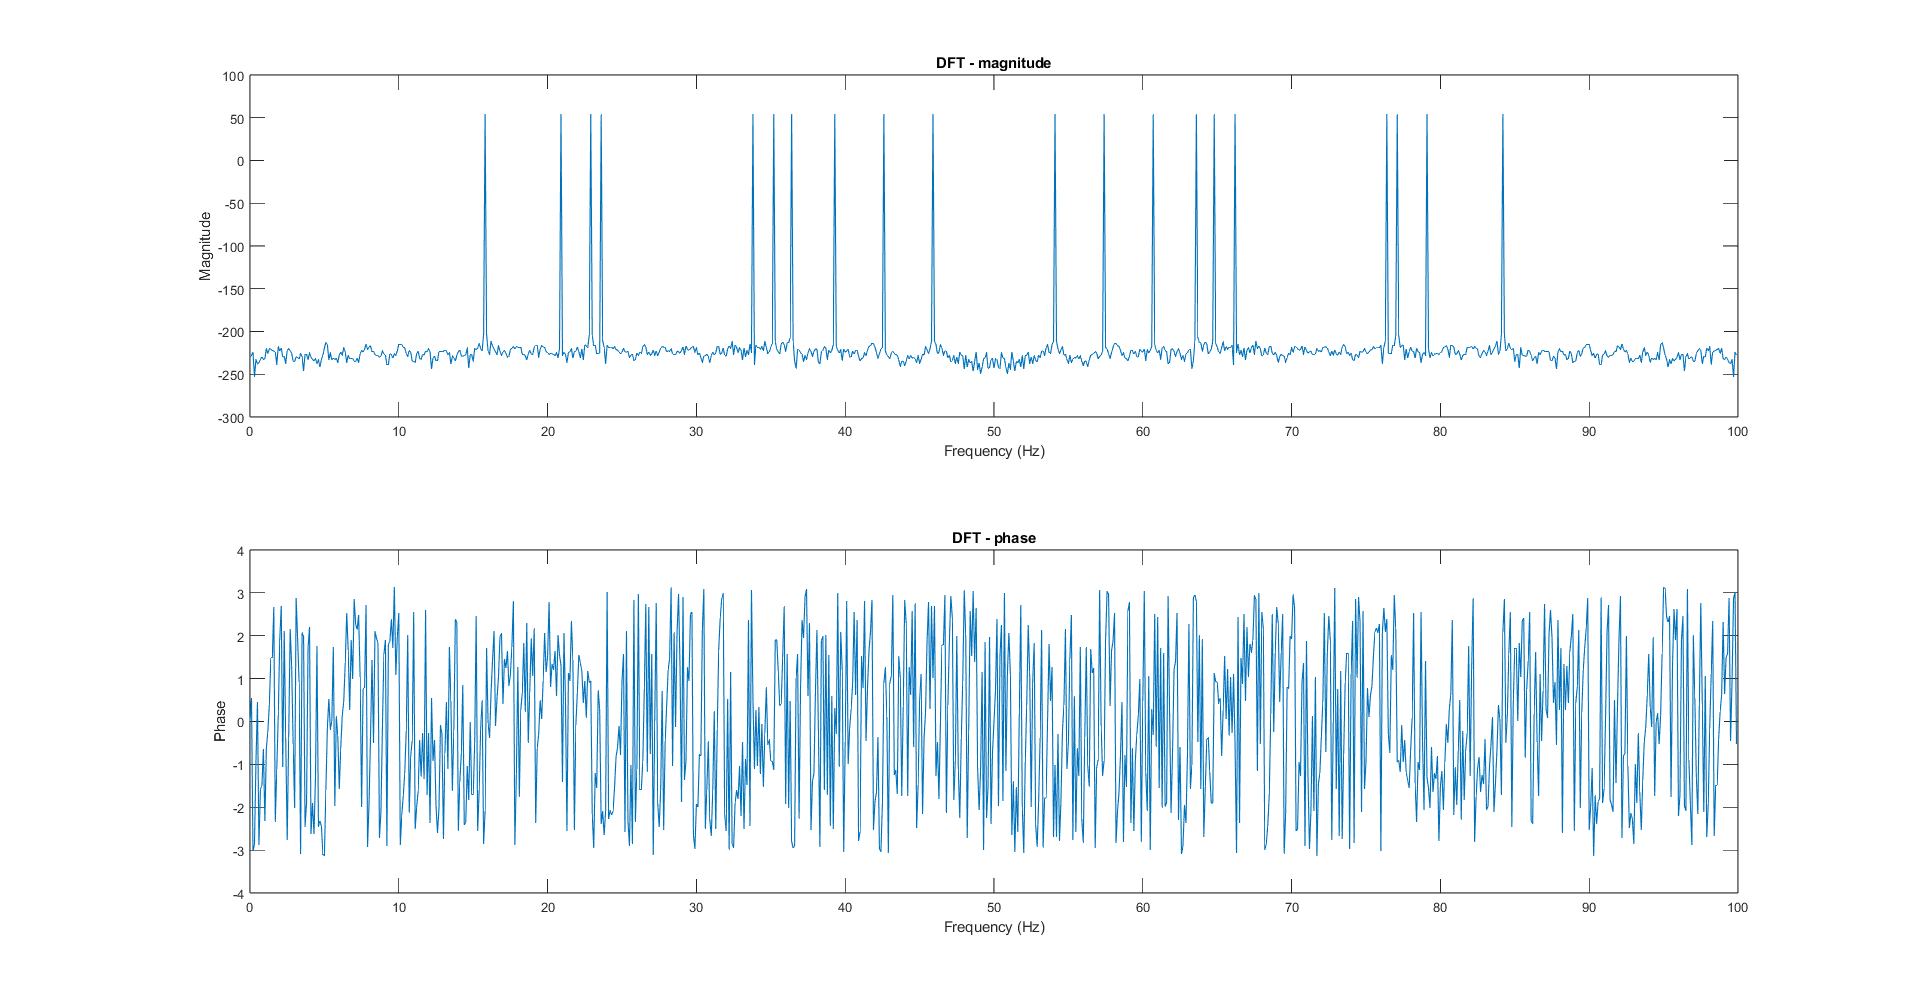
\includegraphics[width=1\textwidth]{part1/task1_3_2.png}
    \caption{Frequency axis in Hz}
\end{figure}

As in task 1.2.5, the frequency axis was converted from bins to Hz by multiplying it by $\omega_1 = \frac{f_s}{N}$.

\begin{Task}{Task 1.3.3. Excite specific frequencies}
    Generate a random phase multisine with a sampling frequency of $200 Hz$, with excited frequencies
    \begin{equation*}
        [4, 8, 12, 16, 20, 24] Hz
    \end{equation*}
    Plot the time and frequency domain results, with appropriate axes.
\end{Task}

\begin{figure}[H]
    \centering
    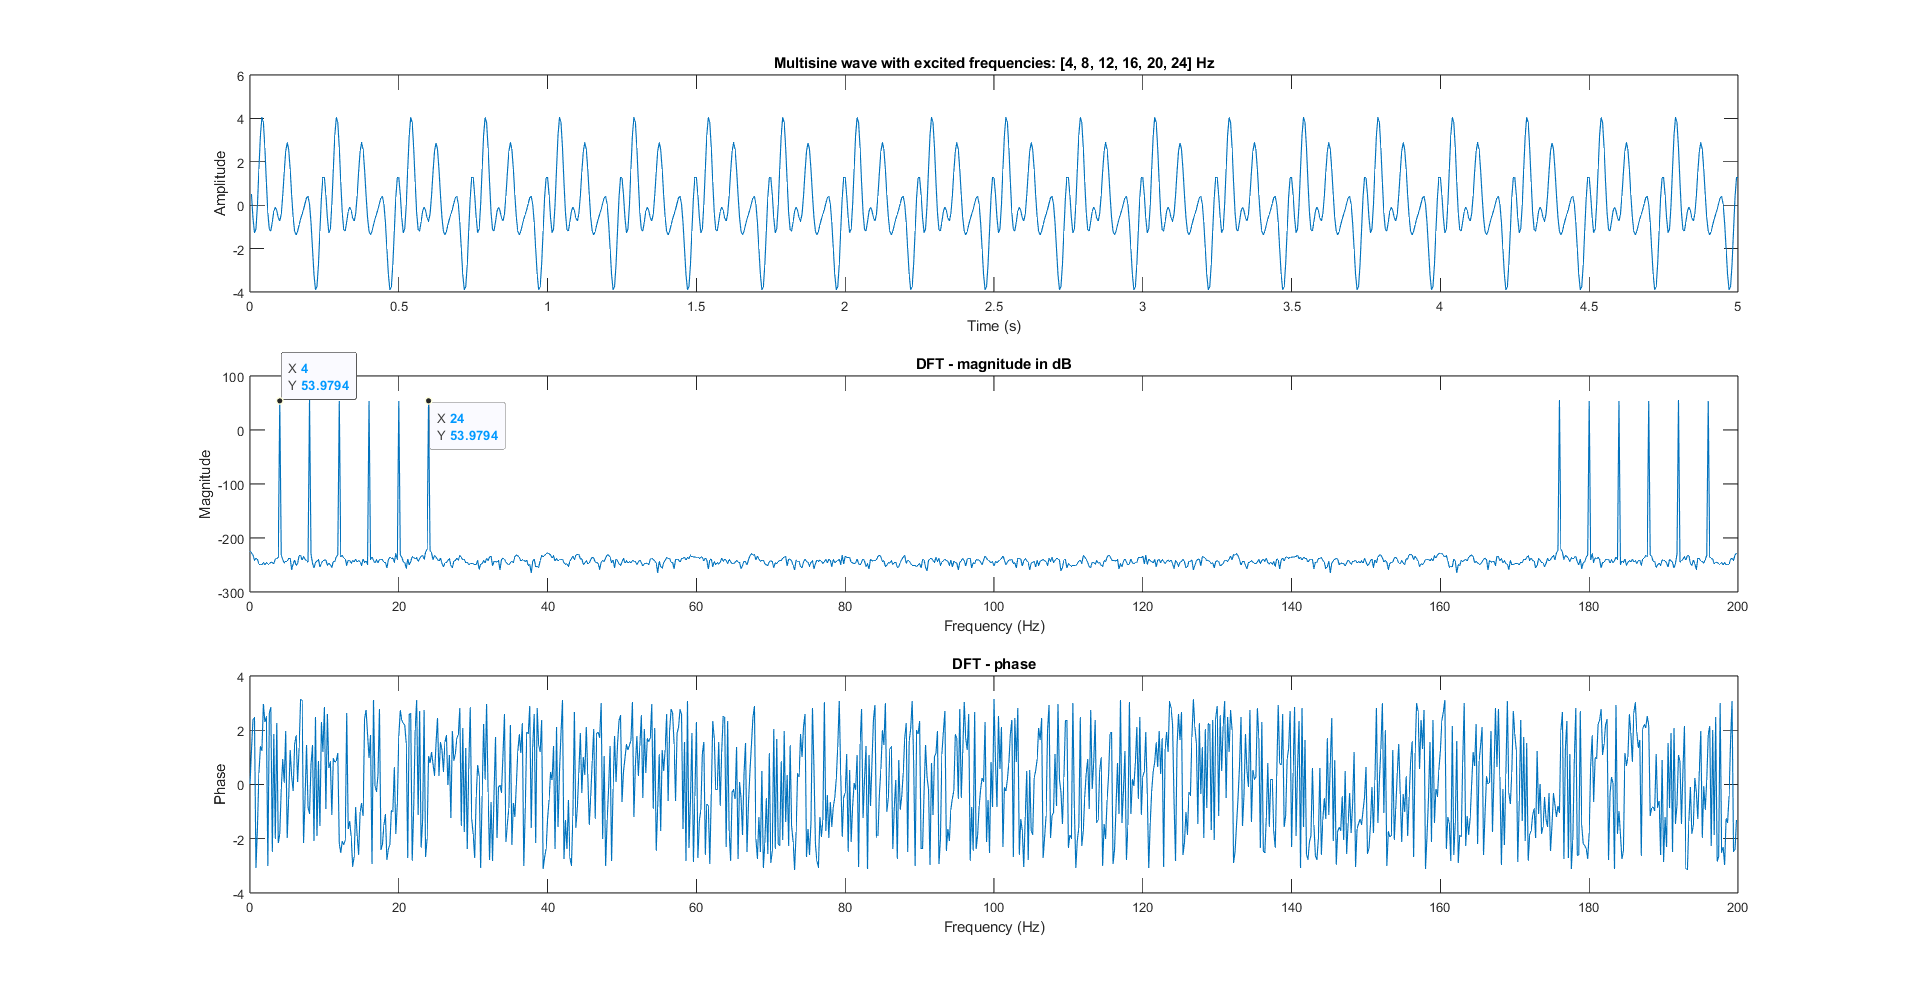
\includegraphics[width=1\textwidth]{part1/task1_3_3.png}
    \caption{Excite specific frequencies}
\end{figure}

\section{Frequency domain construction of a multisine}

\begin{Task}{Task 1.4.1. Trick for frequency domain multisine construction}
    Consider the vector $\tilde{X}(k)$, such that
    \begin{align*}
        \tilde{X}(k) = A_ke^{j\varphi _k} && \text{for} 1 \leq k \leq K\\
        \tilde{X}(k) = 0 && \text{otherwise}
    \end{align*}
    Prove that
    \begin{equation*}
        x(n) = N \Re \left\{\text{iDFT}(\tilde{X}(k))\right\} = \sum_{k = 1}^{K} A_k \cos(\frac{2\pi k}{N} + \varphi_k)
    \end{equation*}
    Where $\Re$ denotes the real part.\\
    \textit{Hint: use the definition of the iDFT}
\end{Task}

Starting from the definition of the iDFT:

\begin{align*}
    x(n) &= \frac{1}{N} \sum_{k=0}^{N-1} X(k) e^{\frac{j 2 \pi k n}{N}}\\
    &= \frac{1}{N} \sum_{k = 1}^{K} A_k e^{j \varphi_k} e^{\frac{j 2 \pi k n}{N}}\\
    &= \frac{1}{N} \sum_{k = 1}^{K} A_k e^{\frac{2\pi k}{N} + \varphi_k}
\end{align*}

By then taking the real part of $x(n)$ and multiplying it by $N$:

\begin{align*}
    x(n) &= \frac{N}{N} \sum_{k = 1}^{K} A_k \Re \left(e^{\frac{2\pi k}{N} + \varphi_k}\right)\\
    &= \sum_{k = 1}^{K} A_k \cos(\frac{2\pi k}{N} + \varphi_k)
\end{align*}

\begin{Task}{Task 1.4.2. Frequency domain multisine}
    Use the frequency domain approach to construct a random phase multisine, by using the trick from Task 1.4.1. Let $N = 1000$, and excite the first $30$ bins. Make time and frequency domain plots (frequency axis expressed in bins).
\end{Task}

\begin{figure}[H]
    \centering
    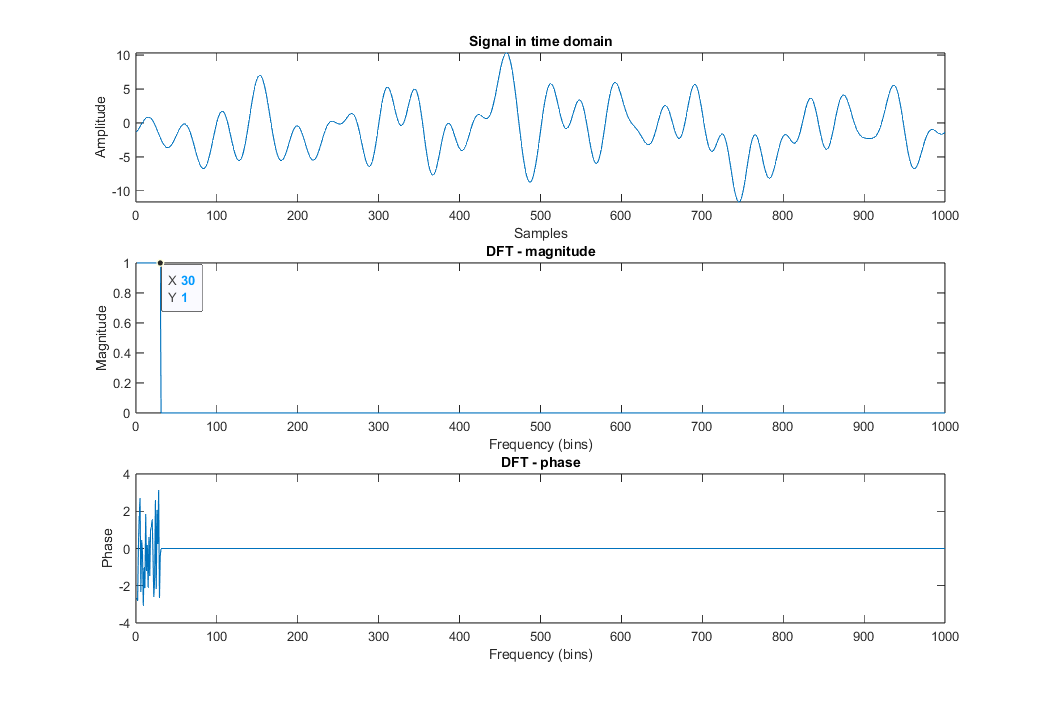
\includegraphics[width=1\textwidth]{part1/task1_4_2.png}
    \caption{Frequency domain multisine}
\end{figure}

\begin{Task}{Task 1.4.3. Specified excited frequency band and frequency resolution}
    Construct a random phase multisine in the frequency domain, which excites the frequency band [5, 15] Hz at 30 equidistantly spaced frequencies. Choose an appropriate sampling frequency. Make time domain and frequency domain plots (time axis in seconds, frequency axis in Hz). How long is one period of this multisine (expressed in seconds)?
\end{Task}

A frequency band of 10 Hz with 30 equidistantly spaced frequencies means that a bin must be equal to $1/3 Hz$ (or a divider of it). Using the formula of $\Delta_f = \frac{f_s}{N}$ (where $\Delta_f$ is the frequency resolution) and using a sampling frequency $f_s$ larger than twice the maximum signal frequency:
\begin{equation*}
    f_s = 50 Hz \quad\quad\quad\quad N = 3 f_s = 150
\end{equation*}

\begin{figure}[H]
    \centering
    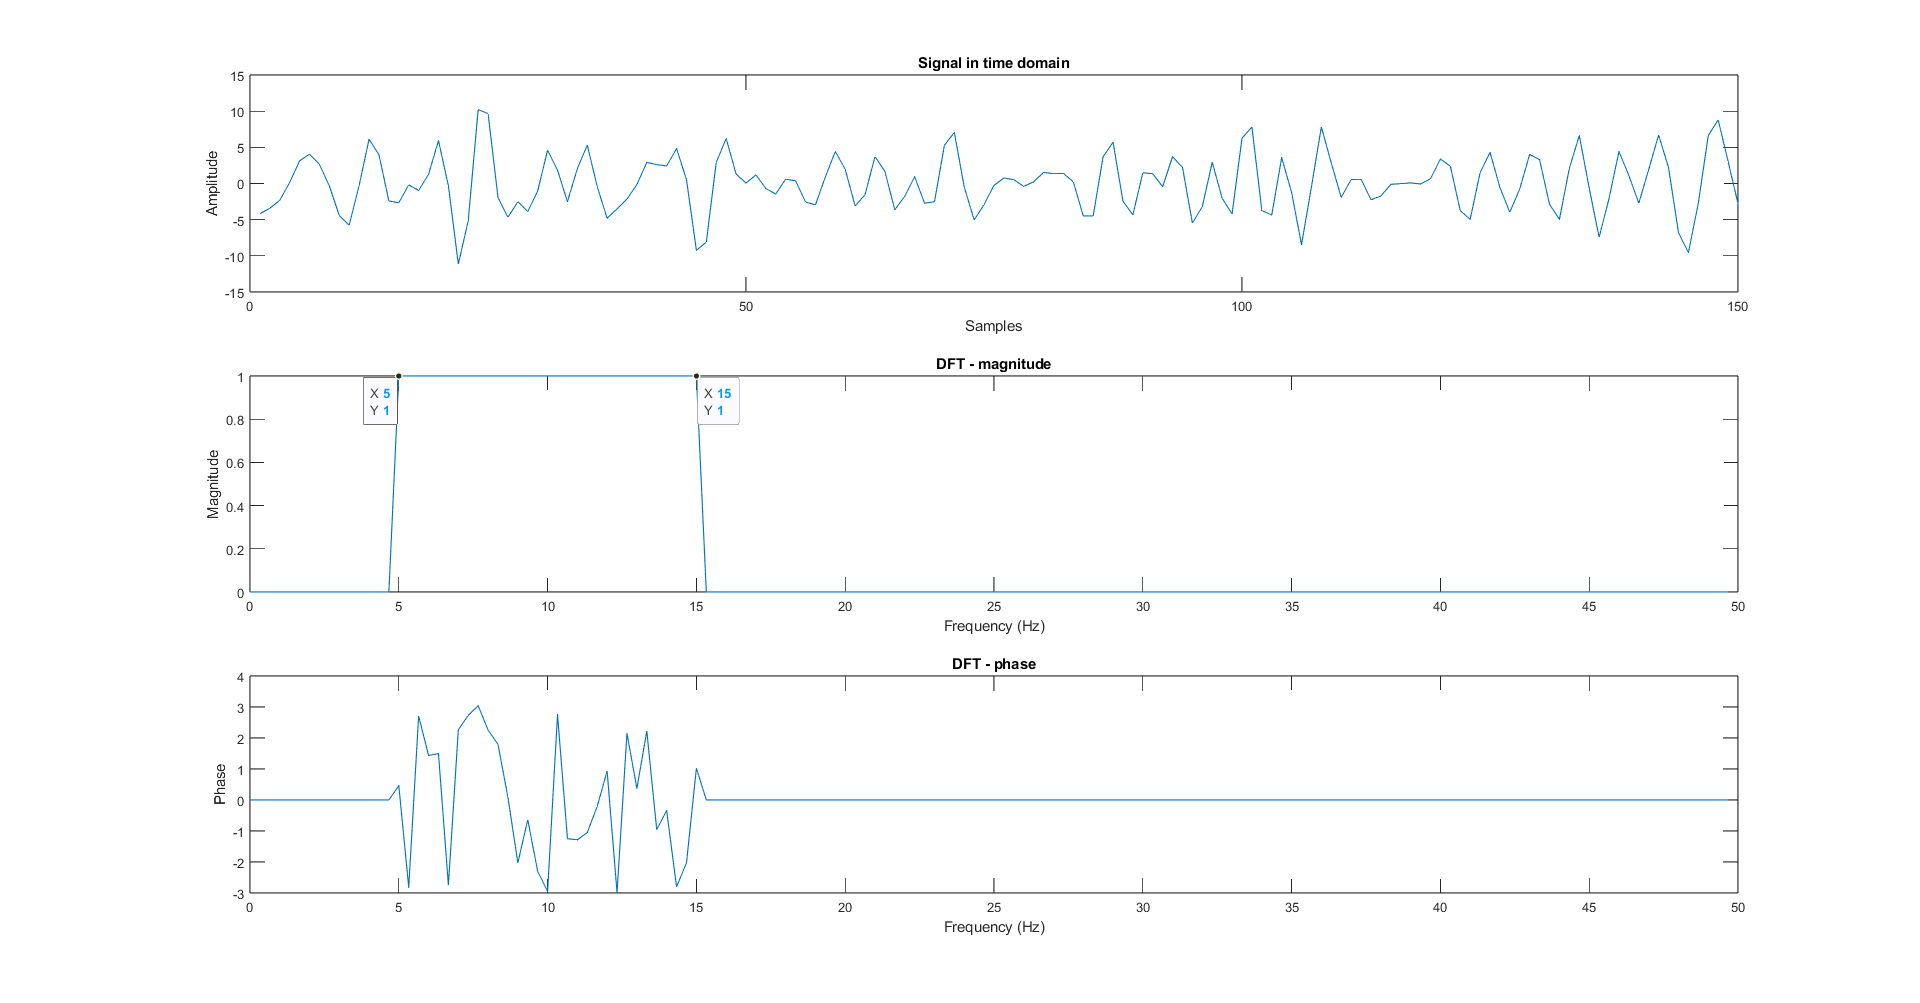
\includegraphics[width=1\textwidth]{part1/task1_4_3.png}
    \caption{Specified excited frequency band and frequency resolution}
\end{figure}

Because it was built with the perfect reconstruction condition, the period of the multisine is equal to the period of a sine at the frequency resolution, which is $1/3 Hz$ so the period is $3$ seconds.

